In the response below, we address the reviewers' comments point-by-point. We want to thank the reviewers for their careful reading of the manuscript and their constructive comments. We have thoroughly revised the manuscript according to the reviewers' suggestions.

%\subsection*{Reviewer 1}
\reviewersection

% \begin{itemize}
%     \item In Definition 2.1, when the model moves to the Gaussian copula, I think the mean parameter becomes redundant and cannot be separated from the transformations. Some comments on this would be helpful.
% \end{itemize}

\begin{point}
    In Definition 2.1, when the model moves to the Gaussian copula, I think the mean parameter becomes redundant and cannot be separated from the transformations. Some comments on this would be helpful.
\end{point}

\begin{reply}
    You are completely right. In fact, this is not the only identifiability issue that the latent Gaussian copula model (LGCM) faces. We added the following lines to the manuscript to address this and related issues:
\end{reply}

% \noindent\textit{You are completely right. In fact, this is not the only identifiability issue that the latent Gaussian copula model (LGCM) faces. We added the following lines to the manuscript to address this and related issues:}

\begin{change}
    %The latent Gaussian copula class suffers from several identifiability issues.
    Several identifiability issues arise in the latent Gaussian copula class.
    First, the mean and the variances are not identifiable unless the monotone transformations \(f\) were restricted to preserve them. Note that this only affects the diagonal entries in \(\mathbf\Sigma\), not the full covariance matrix. Therefore, without loss of generality, we assume the mean to be the zero vector and \(\Sigma_{jj} = 1\) for all \(j \in [d]\). Another identifiability issue relates to the unknown threshold parameters. To ease notation, let \(\Gamma_j^r \equiv f_j(\gamma_j^r)\) and \(\Gamma_j \equiv \{f_j(\gamma_j^r)\}_{r=0}^{l_j+1}\). In the LGCM, only the transformed thresholds \(\Gamma_j\) rather than the original thresholds are identifiable from the discrete variables. We assume, without loss of generality, that the transformed thresholds retain the limiting behavior of the original thresholds, i.e., \(\Gamma_{j}^{0} = -\infty\) and \(\Gamma_j^{l_j+1} = \infty\).
\end{change}


\begin{point}
    The Section 3.2 on nonparanormal case 2 seems very interesting. However, their connection with ML under latent Gaussian model seems a little bit unclear. For example, the likelihood under latent Gaussian is given in eq (3). One natural idea is that, let's try to write down the analog of (3) under the nonparanormal. Of course, this will depend on the unknown function \(f\), but we can plug in the estimator \(\hat{f}\) in Section 3.2. This pseudo-likelihood approach is conceptually reasonable. Is there any connection with the proposed method in current Sec 3.2?
\end{point}

\begin{reply}
    Thank you for pointing us in this direction. We engaged in a short comparison of the two approaches and added the paragraphs below to the Supplementary Materials. Formulating concentration inequalities for this pseudolikelihood approach becomes even more complex due to the polyserial likelihood function's intricate form and the multiple occurrences of the estimated transformations. Therefore, we lead with this empirical study to demonstrate the ad hoc estimator's computational efficiency. However, the pseudolikelihood approach is an interesting avenue for future research.
\end{reply}

\begin{change}
    In this section, we conduct an empirical comparison of \textit{Case II} estimators within the framework of the LGCM. Specifically, we examine the \textit{Case II} MLE derived under the latent Gaussian model, as discussed in Section 2.1 of the Manuscript, which involves incorporating the estimated transformations \(\hat{f}\) at appropriate locations. Furthermore, we investigate the ad hoc estimator presented in Section 3.2 of the Manuscript in more detail.

    We start by rewriting Eq. (6), where we replace occurrences of the $X_k$ with the corresponding transformation $\hat{f}_k(X_k)$. The resulting transformation-based first-order condition (FOC) for the \textit{Case II} MLE under the LGCM becomes:

    \begin{align*}
        \MoveEqLeft \frac{\partial\ell_{jk}^{(n)}(\Sigma_{jk}, x_j^r,\hat{f_k}(x_k))}{\partial \Sigma_{jk}}                                                                                                                                 \\
        = \sum_{i=1}^n & \Bigg[\frac{1}{\Phi(\tilde{\Gamma}_j^{r}(\hat{f_k})) - \Phi(\tilde{\Gamma}_j^{r-1}(\hat{f_k}))}(1-(\Sigma_{jk})^2)^{-\frac{3}{2}}                                                                                  \\
                       & \Big[\phi({\tilde{\Gamma}}_j^{r}(\hat{f_k}))({\Gamma}_j^r\Sigma_{jk} - \hat{f_k}(\tilde{x}_{ik})) - \phi({\tilde{\Gamma}}_j^{r-1}(\hat{f_k}))({\Gamma}_j^{r-1}\Sigma_{jk} - \hat{f_k}(\tilde{x}_{ik}))\Big]\Bigg],
    \end{align*}
    where
    \[\hat{f}_k(\tilde{x}_{ik}) = \frac{\hat{f}_k(x_{ik}) - \hat{f}_k(\bar{x}_k)}{\sqrt{\hat{f}_k(s_k)^2}} \quad \text{and} \quad {\tilde{\Gamma}}_j^{r}(\hat{f}_k) = \frac{{\Gamma}_j^{r} - \Sigma_{jk}\hat{f}_k(\tilde{x}_{ik})}{\sqrt{1-(\Sigma_{jk})^2}}.\]

    In the ensuing empirical evaluation, the data generation scheme is as follows. First, we generate \(n\) data points \((z_{ij}, x_{ik})_{i=1}^n\) from a standard bivariate normal with correlation \(\Sigma^*_{jk}\). Second, we apply the same transformation \(f_t^{-1}(x) = 5x^5\) for \(t \in \{j,k\}\) to all the data points. Third, we generate binary data \(x_{ij}^r\) by randomly choosing \(f^{-1}_j(z_{ij})\)-thresholds (guaranteeing relatively balanced classes) and then applying inversion sampling.

    Computing the transformation-based MLE for \textit{Case II} can be achieved in several ways. Consider the plugged-in log-likelihood function, i.e.,
    \begin{equation*}
        \begin{split}
            \ell_{jk}^{(n)}(\Sigma_{jk}, x_j^r,\hat{f}_k(x_k)) & = \sum_{i=1}^n \big[\log(p(\hat{f}_k(x_{ik}))) + \log(p(x_{j}^{r} \mid \hat{f}_k(x_{ik}), \Sigma_{jk}))\big]                      \\
            & = \sum_{i=1}^n \big[\log(p(\hat{f}_k(x_{ik}))) + \Phi(\tilde{\Gamma}_j^{r}(\hat{f_k})) - \Phi(\tilde{\Gamma}_j^{r-1}(\hat{f_k}))\big].
        \end{split}
    \end{equation*}
    One strategy to optimize the function is direct maximization with a quasi-Newton optimization procedure to determine the optimal values for $\hat\Sigma_{jk}$. This strategy is used, for instance, in the R package \texttt{polycor} \citep{polycor2022}. Alternatively, another approach involves utilizing the FOC and solving for $\hat\Sigma_{jk}$ through a nonlinear root-finding method. To do this, we employ Broyden's method \citep{Broyden1965}.

    In Figure 1, we generate data according to the scheme above for \(n=1000\) and a grid of true correlation values \(\Sigma^*_{jk} \in [0, 0.98]\) with a step size of \(s=0.02\). Due to symmetry, taking only positive correlations is sufficient for comparison purposes. For each correlation value along the grid, we generate \(100\) mixed binary-continuous data pairs and compute the MLE (using the abovementioned strategies) and the ad hoc estimator from Section 3.2 in the main text. We plot the true correlation values against the absolute difference between estimates and true correlation and the corresponding Monte-Carlo standard error for the MLE and the ad hoc estimator.

    \begin{figure}\label{fig:case2_comparison}
        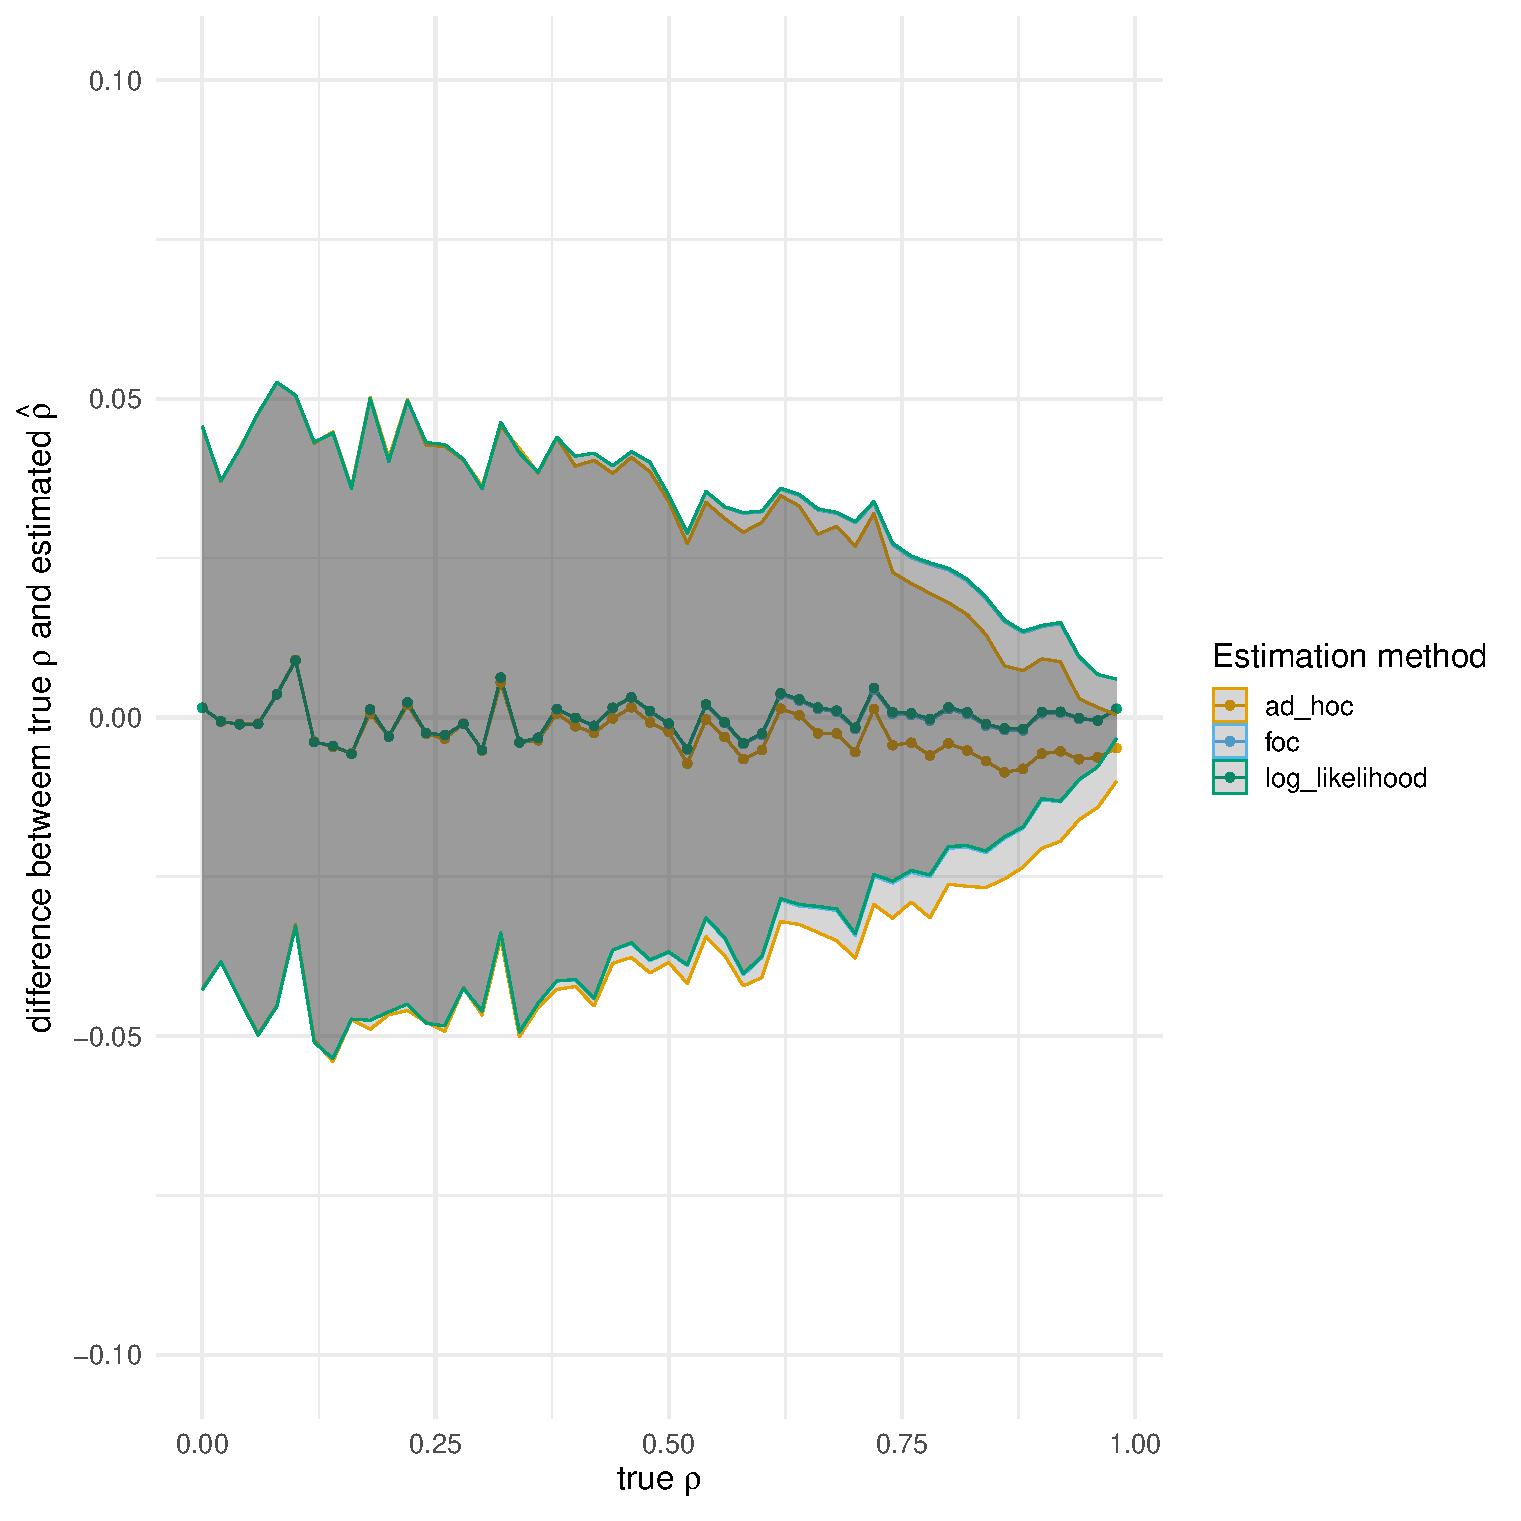
\includegraphics[width=\textwidth]{Figures/case_2_difference.pdf}
        \caption{Comparison of the \textit{Case II} MLE under the LGCM and the ad hoc estimator.}
    \end{figure}

    As expected, both strategies for attaining the MLE yield the same results. The ad hoc estimator's bias becomes noticeable only when the underlying correlation \(\Sigma^*_{jk}\) exceeds \(0.75\) and it remains at such a mild level that we consider it negligible; see \cite{Olsson82} for a similar observation. The strength of the ad hoc estimator lies in its simplicity and computational efficiency. The left panel of Figure 2 shows the median computation time surrounded by the first and third quartiles. We compare the two MLE optimization strategies and the ad hoc estimator for a grid of sample sizes \(n \in [50, 10000]\) with a step size of \(s_t = 50\). Here we fix \(\Sigma^*_{jk} = .87\) and repeat each calculation \(100\) times recording the time elapsed.

    \begin{figure}\label{fig:case2_speed}
        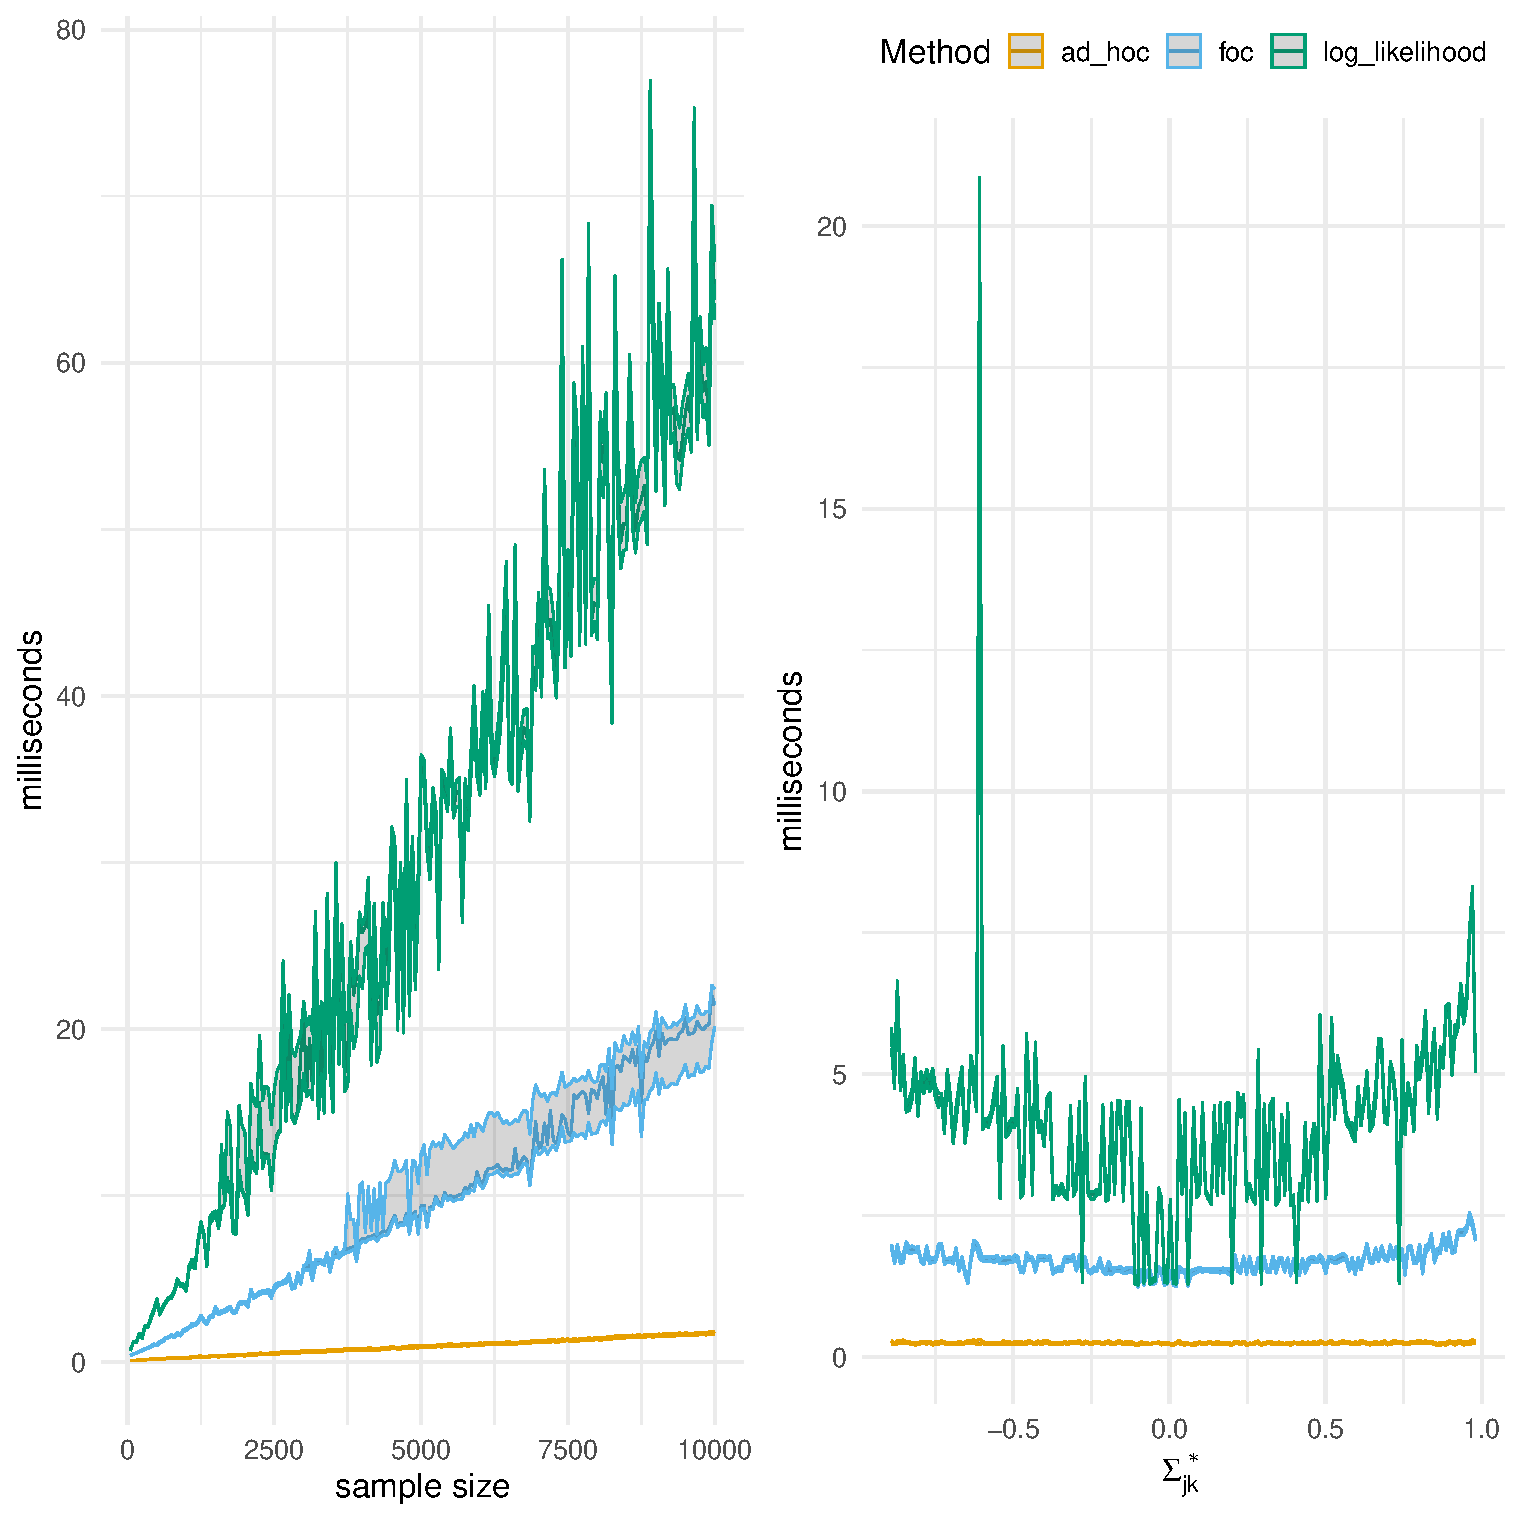
\includegraphics[width=\textwidth]{Figures/case_2_speed_comp.pdf}
        \caption{Computation time in milliseconds for the \textit{Case II} MLE and ad hoc estimators. We report the median (solid line) and the first and third quartile (shaded area) of recorded computation time. In the left panel, we compare computation time against a grid of sample sizes \(n \in [50, 10000]\) with a step size of \(s_t = 50\). In the right panel, we compare computation time against a grid of true correlation values \(\Sigma^*_{jk} \in [-.98, .98]\).}
    \end{figure}

    The right panel of Figure 2 demonstrates computation time across a grid of length \(200\) of values for \(\Sigma_{jk}^* \in [-.98, 98]\). The sample size is, in this case, fixed at \(n=1000\). The ad hoc estimator is consistently and considerably faster than the MLE, regardless of the strategy used. The difference in computation time is especially pronounced for large sample sizes and correlation values approaching the endpoints of the $[-1,1]$-interval. Setting the FOC to zero and solving for \(\Sigma_{jk}\) is computationally more efficient than directly maximizing the log-likelihood function. The time difference in MLE strategies is more pronounced at the endpoints of the $[-1,1]$ interval. The ad hoc estimator is not affected by this issue. Therefore, in the high-dimensional setting we consider in this paper, the ad hoc estimator is preferable to the MLE due to (1) its computational efficiency, (2) its simplicity, which allows us to form concentration inequalities, and (3) its robustness to the underlying correlation value.
\end{change}

\begin{point}
    Theorem 3.2 seems confusing to me. First, it would be more clear if the authors can clarify that this result is for latent Gaussian model (if I am correct). Second, if the right hand side of (14) depends on \(\alpha\), I think the probability of that event on the left hand side should also depend on \(\alpha\), but is not the case in the current formulation. Please clarify this point.
\end{point}

\begin{reply}
    We apologize for the confusion. We clarified the structure of the section and fixed the statement of Theorem 3.2.
\end{reply}

\begin{change}
    The subsequent theorem, drawing on \citet{Mei18}, hinges on four conditions, all substantiated in Section 2 of the Supplementary Materials. This concentration result specifically pertains to the MLEs introduced in Section \ref{sec::latent_gaussian} within the framework of the latent Gaussian model. We remark that related methodology has been applied by \citet{Anne19} in addressing zero-inflated Gaussian data under double truncation.

    \begin{theorem*}
        Suppose that Assumptions \ref{ass1}--\ref{ass3} hold, and let $j \in [d_1]$ and $k \in [d_2]$ for  \textit{Case II} and $j,k \in [d_1]$ for \textit{Case III}. Let $\alpha \in (0,1)$, and let \(n \geq 4 C \log(n) \log\Big(\frac{B}{\alpha}\Big)\) for known constants $B$, $C$, and $D$ depending on cases II and III but independent of $(n,d)$. Then, it holds that
        \begin{equation*}
            P\Bigg(\max_{j,k}\abs{\hat{\Sigma}_{jk}^{(n)} - \Sigma_{jk}^{*}} \geq D\sqrt{\frac{\log(n)}{n} \log\bigg(\frac{B}{\alpha}\bigg)}\Bigg) \leq \frac{d(d-1)}{2}\alpha.
        \end{equation*}
    \end{theorem*}
    \textit{Case I} of the latent Gaussian model addresses the well-understood scenario involving observed Gaussian variables, with concentration results and rates of convergence readily available -see, for example, Lemma 1 in \citet{Ravikumar11}. Consequently, the MLEs converge to \(\mathbf{\Sigma}^{*}\) at the optimal rate of \(n^{-1/2}\), mirroring the convergence rate as if the underlying latent variables were directly observed.
\end{change}

\begin{point}
    It seems that the concentration in Theorem 3.3 is relatively slow, so that one can only obtain the rate \(n^{-1/4}\) rather than the standard \(n^{-1/2}\) (ignoring all log factors). I can expect that the technical analysis is very involved, but it is unclear to me which terms (from estimating \(f\) or other quantities) make the rate slow. Please provide some discussion along this line.
\end{point}

\begin{reply}
    Thanks for raising this issue. We added a discussion on the convergence rate below Corollary 3.4.:
\end{reply}

\begin{change}
    The nonparanormal estimator for \textit{Case II} converges to \(\Sigma_{jk}^*\) at rate \(n^{-1/4}\), which is slower than the optimal parametric rate of \(n^{-1/2}\). This stems not from the presence of the discrete variable but from the direct estimation of the transformation functions \({f}_j\) and the corresponding truncation constant \(\delta_n\). There is room for improvement of the estimator for \(f_j\) to get a rate closer to the optimal one; see \citep{Xue12}. In the numerical analysis below, we find that Theorem \ref{concentration_caseII} gives a worst-case rate that does not appear to negatively impact performance compared to estimators that attain the optimal rate.
\end{change}


\reviewersection

\begin{point}
    \textbf{Threshold estimation}: As the authors noted, the two-step estimation procedure relies crucially on the estimation of the unknown thresholds which map the latent Gaussian variable to the observed ordinal variable. The quantile estimator in 3.4 makes sense but I cannot see how Lemma 3.1 “assures that these threshold estimates can be formed with high accuracy.” Lemma 3.1 seems to say that the estimators are bounded away from infinity with high probability. Maybe I’m missing some important connections here. In addition, I assume \(A^{cj}\) stands for the complement of \(
    A^j\), i.e. \((A^j)^c\).
\end{point}

\begin{reply}
    You are right; the connection between Lemma 3.1 and the threshold estimation was unclear. We fixed the statement accordingly.
\end{reply}

\begin{change}
    The following lemma assures that the threshold estimates can be formed with high accuracy.
    \begin{lemma}\label{lemma::thresholds}
        Suppose the estimated thresholds are bounded away from infinity, i.e., \(\Abs{\hat\Gamma^r_j} \leq G\) for all $j \in [d_1]$ and $r = 1, \dots, l_j$ and some \(G\). The following bound holds for all $t > 0$ with Lipschitz constant \(L_1 = 1/(\sqrt{\frac{2}{\pi}} \min\{\hat\pi^r_j, 1- \hat\pi^r_j\})\):
        \begin{equation*}
            P\Big(\Abs{\hat\Gamma_j^r - \Gamma_j^r} \geq t \Big) \leq 2\exp{\Big(- \frac{2t^2n}{L_1^2}\Big)}.
        \end{equation*}
    \end{lemma}

    The proof of Lemma \ref{lemma::thresholds} is given in Section 5 %\ref{lemma_threshold_proof}%
    of the Supplementary Materials. The requirement that the estimated thresholds are bounded away from infinity typically does not pose any restriction in finite samples. All herein-developed methods are applied in a two-step fashion. In the ensuing theoretical results, we stress this by denoting the estimated thresholds as $\bar{\Gamma}_j^r$.
\end{change}


\begin{point}
    \textbf{Concentration results}: Given that this manuscript is proposing a unifying model for mixed graphical models, it might help the readers if the authors can compare the rates in Theorems 3.2 and 3.3 with existing rates in special cases. In particular, (i) the concentration inequality (14) should match existing rates for Gaussian graphical models when plugging in proper \(\alpha\), and (ii) the five terms in the probability bound in Theorem 3.3 can use some explanation.
\end{point}

\begin{reply}
    Thanks for the suggestion. We added a comparison of the concentration results to the existing rates for Gaussian graphical models. We also discuss the suboptimal rate of convergence in Theorem 3.3. As we mention below, there is room for improvement of the estimator for \(f_j\) to get a rate closer to the optimal one. This is something we are currently investigating further.
\end{reply}

\begin{change}
    \begin{theorem*}
        Suppose that Assumptions \ref{ass1}--\ref{ass3} hold, and let $j \in [d_1]$ and $k \in [d_2]$ for  \textit{Case II} and $j,k \in [d_1]$ for \textit{Case III}. Let $\alpha \in (0,1)$, and let \(n \geq 4 C \log(n) \log\Big(\frac{B}{\alpha}\Big)\) for known constants $B$, $C$, and $D$ depending on cases II and III but independent of $(n,d)$. Then, it holds that
        \begin{equation*}
            P\Bigg(\max_{j,k}\abs{\hat{\Sigma}_{jk}^{(n)} - \Sigma_{jk}^{*}} \geq D\sqrt{\frac{\log(n)}{n} \log\bigg(\frac{B}{\alpha}\bigg)}\Bigg) \leq \frac{d(d-1)}{2}\alpha.
        \end{equation*}
    \end{theorem*}
    \textit{Case I} of the latent Gaussian model addresses the well-understood scenario involving observed Gaussian variables, with concentration results and rates of convergence readily available -see, for example, Lemma 1 in \citet{Ravikumar11}. Consequently, the MLEs converge to \(\mathbf{\Sigma}^{*}\) at the optimal rate of \(n^{-1/2}\), mirroring the convergence rate as if the underlying latent variables were directly observed.
\end{change}

\begin{change}
    The first four terms in the probability bound stem from finding bounds to different regions of the support of the transformed continuous variable. The last term is a consequence of the fact that we estimate the transform directly.

    The nonparanormal estimator for \textit{Case II} converges to \(\Sigma_{jk}^*\) at rate \(n^{-1/4}\), which is slower than the optimal parametric rate of \(n^{-1/2}\). This stems not from the presence of the discrete variable but from the direct estimation of the transformation function \({f}_j\) and the corresponding truncation constant \(\delta_n\). Both \citet{Xue12} and \citet{Liu12} discuss room for improvement of the estimator for \(f_j\) to get a rate closer to the optimal one. In the numerical analysis below, we find that Theorem \ref{concentration_caseII} gives a worst-case rate that does not appear to negatively impact performance compared to estimators that attain the optimal rate.
\end{change}

\begin{point}
    \textbf{Numerical Experiments}: It seems that too many details are deferred to the supplementary materials that a reader cannot understand how the data are simulated by reading the main text. If space is of concern, the two tables can be condensed into two plots. Furthermore, some rows (e.g., TPR and FPR) can be deferred to the supplementary materials as there are no additional insights to learn from these numbers. In addition, the real data analysis can also be deferred to the supplementary materials. I fail to gain any new insights about Covid from this analysis, and the texts in Fig. 1 and 2 are too small to read. The data analysis can be improved, but, in my opinion, it serves only as a distraction to the paper considering that the main contribution of this paper is a general model. Lastly, the low number of replicates in simulation (100 in Tables 1 and 2) makes me concern about the computational feasibility of the proposed method. Maybe the authors can report the computing time, as this might give more insight into the proposal’s computational feasibility.
\end{point}

\begin{reply}
    Thanks again for the helpful suggestions. We agree with your points and thus condensed the tables into plots and moved some of the details to the Supplementary Materials, including the real data analysis. We added the simulation setup back to the main text. The low number of replicates in the simulation study has been set due to the \(d=750\) scenario. Calculating \({750\choose 2}\) correlation pairs, plugging the corresponding correlation matrix into the \textit{glasso} routine for each penalty parameter \(\lambda\) along a grid of length 30 for four different estimators is computationally expensive. We added a microbenchmark of the correlation matrix estimation to give an idea of the computational feasibility of the proposed and existing methods. When applied in practice, one typically only runs the procedure once for a given dataset.
\end{reply}

\begin{change}
    Below, we provide a small microbenchmark study regarding the computational feasibility of the proposed and existing methods. We compare the computation time of the correlation matrix estimation for the \texttt{oracle} estimator \cite{Liu12}, our proposed polyserial/polychoric method, and the \texttt{bridge} ensemble estimator \cite{Feng19}. The results are displayed in Table \ref{table::timing}.

    \begin{table}[htbp!]
        \caption{Microbenchmark of the correlation matrix estimation. Displayed are mean compute times of the correlation matrix of the general mixed simulation setup described in Section \ref{sec::setup} for the \texttt{oracle} estimator, our proposed polyserial/polychoric method, and the \texttt{bridge} ensemble estimator.}

        \begin{center}
            
\begin{tabular}{lrr}
    \toprule
    Method & Dimension & Time (s)   \\
    \midrule
    oracle & 50        & 0.2947     \\
    poly   & 50        & 58.4005    \\
    bridge & 50        & 181.6449   \\
    \addlinespace
    oracle & 250       & 6.6614     \\
    poly   & 250       & 1487.8901  \\
    bridge & 250       & 4761.2884  \\
    \addlinespace
    oracle & 750       & 66.9916    \\
    poly   & 750       & 9102.1628  \\
    bridge & 750       & 27789.9450 \\
    \bottomrule
\end{tabular}
        \end{center}
        \label{table::timing}
    \end{table}

    The general mixed data simulation setup we use here is detailed in Section \ref{sec::setup}. We report the mean computation time in seconds over \(20\) repetitions. The \texttt{oracle} estimator is the fastest, followed by the polyserial/polychoric method and the \texttt{bridge} ensemble estimator. Computing polyserial/polychoric correlations is about three times faster than the bridge function approach. In the \(d=750\) setting, our polyserial/polychoric method takes, on average, around 2.5 hours to compute the correlation matrix. The \texttt{bridge} ensemble estimator requires about 7.7 hours.
\end{change}